% TEMPLATE for Usenix papers, specifically to meet requirements of
%  USENIX '05
% originally a template for producing IEEE-format articles using LaTeX.
%   written by Matthew Ward, CS Department, Worcester Polytechnic Institute.
% adapted by David Beazley for his excellent SWIG paper in Proceedings,
%   Tcl 96
% turned into a smartass generic template by De Clarke, with thanks to
%   both the above pioneers
% use at your own risk.  Complaints to /dev/null.
% make it two column with no page numbering, default is 10 point

% Munged by Fred Douglis <douglis@research.att.com> 10/97 to separate
% the .sty file from the LaTeX source template, so that people can
% more easily include the .sty file into an existing document.  Also
% changed to more closely follow the style guidelines as represented
% by the Word sample file.

% Note that since 2010, USENIX does not require endnotes. If you want
% foot of page notes, don't include the endnotes package in the
% usepackage command, below.

% This version uses the latex2e styles, not the very ancient 2.09 stuff.
\documentclass[letterpaper,twocolumn,10pt]{article}

% There is a minted package for lang syntax highlighting. But, I didn't like the
% colored output.
\usepackage{url,epsfig,endnotes,authblk,amsmath,algorithm,algpseudocode}

% \usepackage[scaled=0.95]{inconsolata}
% \renewcommand*\familydefault{\ttdefault} %% Only if the base font of the document is to be typewriter style

% This is a fonts package. For now, not bothering with it.
% \usepackage[T1]{fontenc}
% \usepackage{tgbonum}

\usepackage[sc]{mathpazo}

% \usepackage[switch]{lineno}
% Using above, plus adding \linenumbers after begin document would add line
% numbers on both sides.

\usepackage{usenix2019_v3}
% \setlength{\columnsep}{1cm}

\newcommand{\uid}{\textit{uid} }
\newcommand{\uids}{\textit{uids} }

\begin{document}
%don't want date printed
\date{}

%make title bold and 14 pt font (Latex default is non-bold, 16 pt)
\title{\Large \bf Dgraph: Synchronously Replicated, Transactional and Distributed Graph Database}

\author{Manish Jain}
\affil{\texttt {manish@dgraph.io}}
\affil{Dgraph Labs, Inc.}
\affil{Version: 0.8 Last Updated: \today}

\maketitle

% Use the following at camera-ready time to suppress page numbers.
% Comment it out when you first submit the paper for review.
% \thispagestyle{empty}

\subsection*{Abstract}

Dgraph is a distributed graph database which provides horizontal scalability,
distributed cluster-wide ACID transactions, low-latency arbitrary-depth joins,
synchronous replication, high availability and crash resilience.  Aimed at
real-time transactional workloads, Dgraph shards and stores data in a way to
optimize joins and traversals, while still providing data retrieval and
aggregation. Dgraph's unique take is to provide low-latency arbitrary-depth
joins in a constant number of network calls (typically, just one network call)
that would be required to execute a single join, irrespective of the size of the
cluster or the size of the result set.

\section{Introduction}

Distributed systems or databases tend to suffer from join depth problem. That
is, as the number of traversals of relationships increase within a query, the
number of network calls required (in a sufficiently sharded dataset) increase.
This is typically due to entity-based data sharding, where entities are randomly
(sometimes with a heuristic) distributed across servers containing all the
relationships and attributes along with them. This approach suffers from
high-fanout result set in intermediate steps of a graph query causing them to do
a broadcast across the cluster to perform joins on the entities. Thus, a single
graph query results in network broadcasts, hence causing a jump in the query
latency as the cluster grows.

Dgraph is a distributed database with a native graph backend. It is the only
native graph database to be horizontally scalable and support full
ACID-compliant cluster-wide distributed transactions. In fact, Dgraph is the
first graph database to have been Jepsen\cite{jepsen} tested for transactional
consistency.

Dgraph automatically shards data into machines, as the amount of data or the
number of servers change, and automatically reshards data to move it across
servers to balance the load.  It also supports synchronous replication backed by
Raft\cite{raft} protocol, which allows the queries to seamlessly failover to
provide high availability.

Dgraph solves the join depth problem with a unique sharding mechanism. Instead
of sharding by entities, as most systems do, Dgraph shards by
relationships.  Dgraph's unique way of sharding data is inspired by research at
Google\cite{latency}, which shows that the overall latency of a query is greater
than the latency of the slowest component. The more servers a query touches to
execute, the slower the query latency would be. By doing relationship based
sharding, Dgraph can execute a join or traversal in a single network call (with
a backup network call to replica if the first is slow), irrespective of the size
of the cluster or the input set of entities. Dgraph executes arbitrary-depth
joins without network broadcasts or collecting data in a central place. This
allows the queries to be fast and latencies to be low and predictable.

\section{Dgraph Architecture} \label{arch}

Dgraph consists of Zeros and Alphas, each representing a group that they are
serving. Zeros serve group zero and Alphas serve group one, group two and
onwards. Each group forms a Raft cluster of 1, 3 or 5 members configurable by a
human operator (henceforth, referred to as the operator). All updates made to
the group are serialized via Raft consensus algorithm and applied in that order
to the leader and followers.

Zeros store and propagate metadata about the cluster while Alphas store user
data. In particular, Zeros are responsible for membership information, which
keeps track of the group each Alpha server is serving, its internal IP address
for communication within the cluster, the shards it is serving, etc. Zeros do
not keep track of the health of the Alphas and take actions on them -- that is
considered the job of the operator. Using this information, Zero can tell the new
Alpha to either join and serve an existing group, or form a new group.

The membership information is streamed out from Zero to all the Alphas. Alphas
can use this membership information to route queries (or mutations) which hit
the cluster. Every instance in the cluster forms a connection with every other
instance (thus forming $2 \times \binom{N}{2}$ open connections, where N =
number of Dgraph instances in the cluster), however, the usage of this
connection depends on their relationship. For example, a Raft leader-follower
relationship would have heartbeats (every 100 ms) and data flowing, while an
Alpha would only talk to Alpha in another group when it needs to do so for
processing queries or mutations. Every open connection does have light-weight
health checks to avoid stalling on a target server which has become unresponsive
(died, partitioned, etc.). Both Alphas and Zeros expose one port for
intra-cluster communication over Grpc\cite{grpc} and one for external communication with
clients over HTTP. Alphas additionally expose an external Grpc port for
communication with Grpc based clients -- all official clients run over Grpc.

\begin{figure}[t]
\begin{center}
	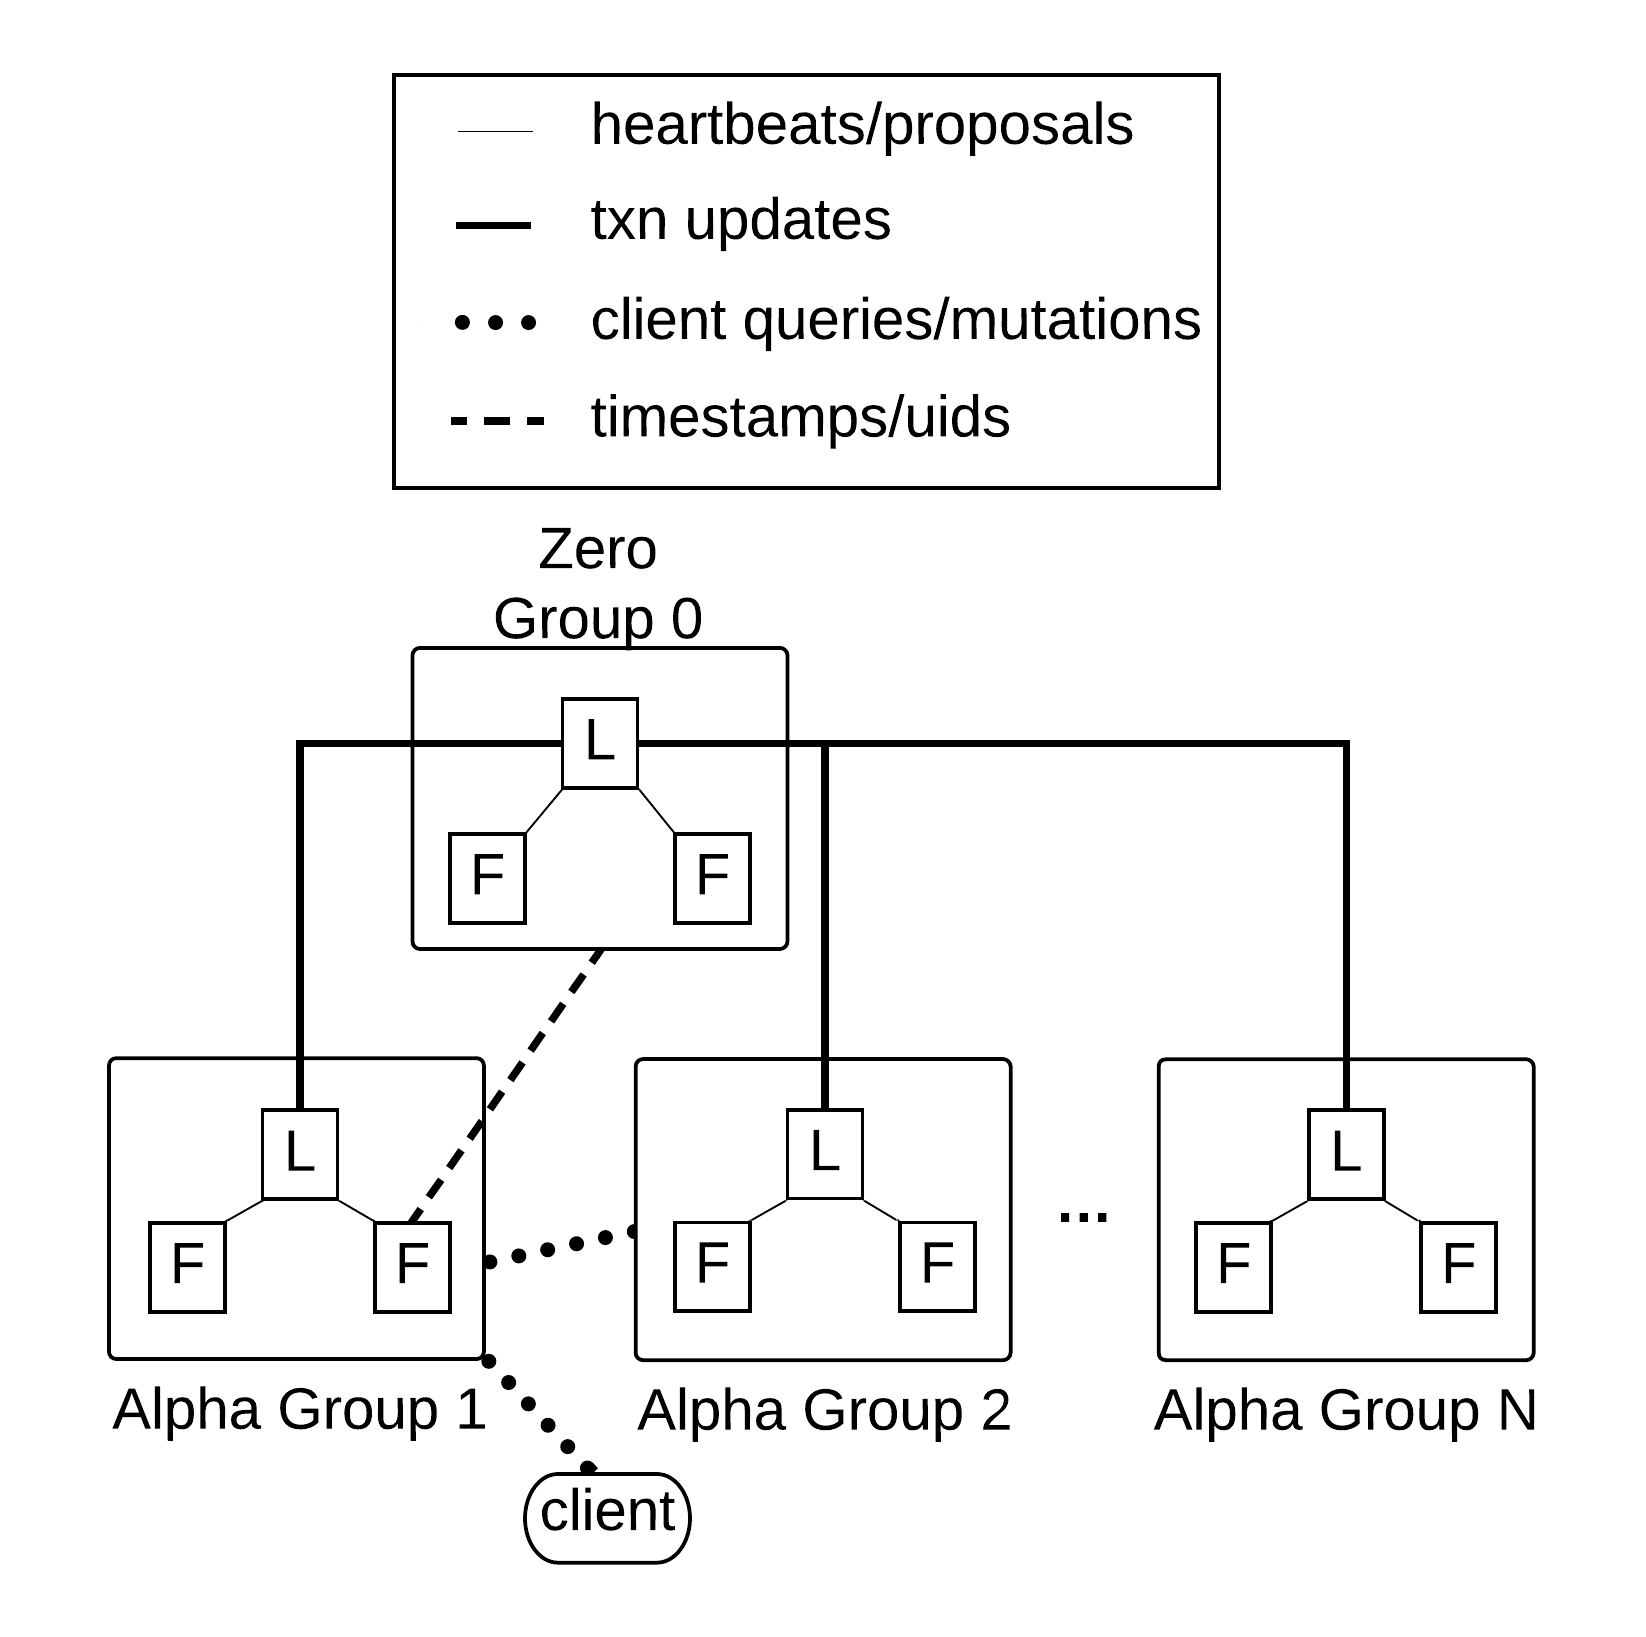
\includegraphics[scale=0.5]{architecture.png}
\end{center}
\caption{Dgraph Architecture: There is one Zero group and multiple Alpha
groups. Each group is a Raft group consisting of one or more members.}
\end{figure}

Zero also runs an oracle which hands out monotonically-increasing logical
timestamps for transactions in the cluster (no relation to system time). A Zero
leader would typically lease out a bandwidth of timestamps upfront via Raft
proposal and then service timestamp requests strictly from memory without any
further coordination. Zero oracle tracks additional things for aiding with
transaction commits, which would be elaborated in section \ref{txn}.

Zero gets information about the size of data in each group from the Alpha leaders,
which it uses to make decisions about shard movement, which would be elaborated
in section \ref{move}.


\subsection{Data Format}

Dgraph can input data in a JSON format or (slightly modified) RDF NQuad format.
Dgraph would break down a JSON map into smaller chunks, with each JSON key-value
forming one record equivalent of a single RDF triple record. When parsing RDF
Triple or JSON, data is directly converted into an internal protocol buffer
\cite{protobuf} data format and not interchanged among the two.

\begin{verbatim}

{
  "uid"   : "0xab",
  "type"  : "Astronaut",
  "name"  : "Mark Watney",
  "birth" : "2005/01/02",
  "follower": { "uid": "0xbc", ... },
}

<0xab> <type>  "Astronaut" .
<0xab> <name>  "Mark Watney" .
<0xab> <birth> "2005/01/02" .
<0xab> <follower> <0xbc> .

\end{verbatim}

A triple is typically expressed as a subject-predicate-object or a
subject-predicate-value. Subject is a node, predicate is a relationship, and
object can be another node or a primitive data type. One points from a node to
another node, the other points from a node to a value. In the above example, the
triple with name is a type of subject-predicate-value (typically referred to as
an attribute), while the triple with follower is a type of
subject-predicate-object. Dgraph makes no difference in how it handles these two
types of records (to avoid confusion over these two types, we'll refer to them
as object-values). Dgraph considers this as the unit of record and a typical
JSON map would be broken into multiple such records.

Data can be retrieved from Dgraph using GraphQL\cite{gql} and a modified version of
GraphQL, called GraphQL+-\cite{dgql}. GraphQL+- has most of the same
properties as GraphQL. But, adds various properties which are important for a
database, like query variables, functions and blocks. More information about how
the query language came to be and the differences between GraphQL and GraphQL+-
can be found in this blog post \cite{gqldb}.

As mentioned in section \ref{arch}, all internal and external communication in
Dgraph runs via Grpc and Protocol Buffers. Dgraph also exposes HTTP endpoints to
allow building client libraries in languages which are not supported by these
two.  There is a functionality parity between HTTP endpoints and APIs exposed
via Grpc.

In accordance with the GraphQL spec, query responses from Dgraph are in JSON
format, both over HTTP and Grpc.

\subsection{Data Storage} \label{storage}

Dgraph data is stored in an embeddable key-value database called
Badger\cite{badger} for data input-output on disk. Badger is an LSM-tree based
design, but differs from others in how it can optionally store values separately
from keys to generate a much smaller LSM tree, which results in both lower write
and read amplification. Various benchmarks run by the team show Badger to
provide equivalent or faster writes than other LSM based DBs, while providing
equivalent read latencies compared to B+-tree based DBs (which tend to provide
much faster reads than LSM trees).

As mentioned above, all records with the same predicate form one shard. Within a
shard, records sharing the same subject-predicate are grouped and condensed into
one single key-value pair in Badger. This value is referred to as a
\textbf{posting list}, a terminology commonly used in search engines to refer to
a sorted list of doc ids containing a search term. A posting list is stored as a
value in Badger, with the key being derived from subject and predicate.

\begin{verbatim}
<0x01> <follower> <0xab> .
<0x01> <follower> <0xbc> .
<0x01> <follower> <0xcd> .
...
key = <follower, 0x01>
value = <0xab, 0xbc, 0xcd, ...>
\end{verbatim}

All subjects in Dgraph are assigned a globally unique id, called a \uid. A
\uid is stored as a 64-bit unsigned integer (uint64) to allow efficient, native
treatment by Go language in the code base. Zero is responsible for handing out
\uids as needed by the Alphas and does it in the same monotonically increasing
fashion as timestamps (section \ref{arch}). A \uid once allocated is never
reallocated or reassigned. Thus, every node in the graph can be referenced by a
unique integer.

Object-values are stored in postings. Each posting has an integer id. When the
posting holds an object, the id is the \uid assigned to that object. When posting
holds a value, the integer id for value is determined based upon the schema of
the predicate. If the predicate allows multiple values, the integer id for the
value would be a fingerprint of the value. If the predicate stores values with
language, the integer id would be a fingerprint of the language tag. Otherwise,
the integer id would be set to maximum possible uint64 (2\textsuperscript{64} -
1). Both \uid and integer id is never set to zero.

Value could be one of the many supported data types: int, float, string,
datetime, geo, etc. The data is converted into binary format and stored in a
posting along with the information about the original type. A posting can also
hold facets. Facets are key-value labels on an edge, treated like attachments.

In a common case where the predicate only has objects (and no values like
follower edge), a posting list would consist largely of sorted \uids. These are
optimized by doing integer compression. The \uids are grouped in blocks of 256
integers (configurable), where each block has a base \uid and a binary blob. The
blob is generated by taking a difference of current \uid with the last and
storing the difference in bytes encoded using group varint. This generates a
data compression ratio of 10. When doing intersections, we can use these blocks
to do binary searches or block jumps to avoid decoding all the blocks. Sorted
integer encoding is a hotly researched topic and there is a lot of room for
optimization here in terms of performance. Work is going on currently to use
Roaring Bitmaps\cite{roaring} instead to represent this data.

\begin{figure}[t]
\begin{center}
	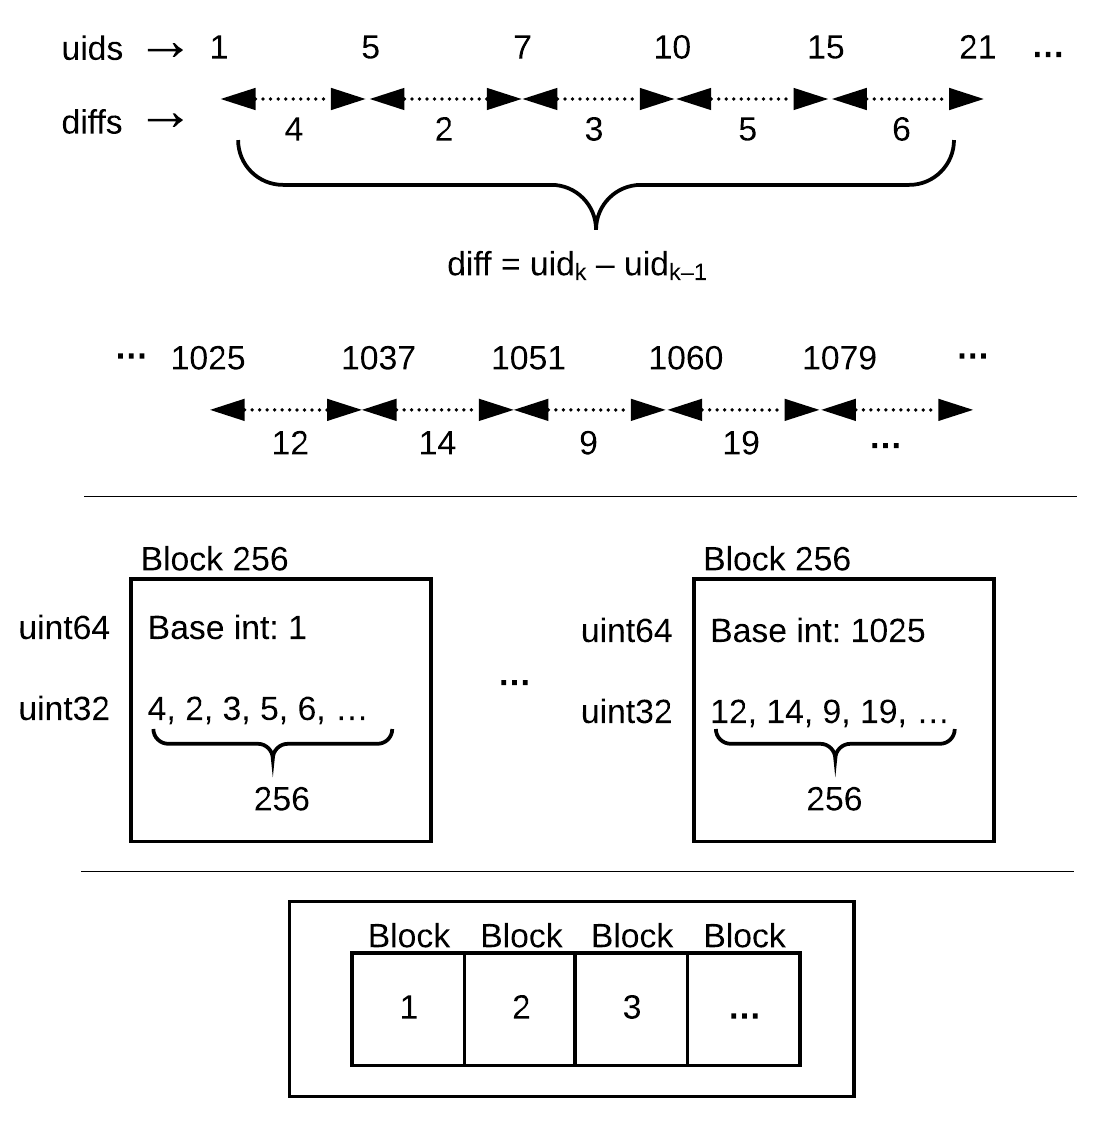
\includegraphics[scale=0.8]{integerstorage.png}
\end{center}
\caption{Posting list structure stored in group varint-encoded blocks}
\end{figure}

Thanks to these techniques, a single edge traversal corresponds to only a single
Badger lookup. For example, finding a list of all of X's followers would involve
doing a lookup on \texttt{<follower, X>} key which would give a posting list containing
all of their followers' \uids. Further lookups can be made to get a list of posts
made by followers . Common followers between X and Y an be found by doing two
lookups followed by intersecting the sorted int lists of \texttt{<follower, X>} and
\texttt{<follower, Y>}. Note that distributed joins and (object based) traversals only
require \uids to be transmitted over network, which is also very efficient. All
this allows Dgraph to be very efficient on these operations, without
compromising on the typical \texttt{select * from table where X=Y} style record lookups.

This type of data storage has benefits in joins and traversals, but comes with
an additional problem of high fan-out. If there are too many records with the
same \texttt{<subject, predicate>}, the overall posting list could grow to an
untenable size. This is typically only a problem for objects (not so much for
values). We solve this by binary splitting a posting list as soon as its on-disk
size hits a certain threshold. A split posting list would be stored as multiple
keys in Badger, with optimizations made to avoid retrieving the splits until the
operation needs them. Despite storage differences, the posting list continues to
provide the same sorted iteration via APIs as an unsplit list.

\subsection{Data Sharding}

While Dgraph shares a lot of features of NoSQL and distributed SQL databases, it
is quite different in how it handles its records. In other databases, a row or
document would be the smallest unit of storage (guaranteed to be located
together), while sharding could be as simple as generating equal sized chunks
consisting of many of these records.

Dgraph's smallest unit of record is a triple (subject-predicate-object,
described below), with each predicate in its entirety forming a shard. In other
words, Dgraph logically groups all the triples with the same predicate and
considers them one shard.  Each shard is then assigned a group (1..N) which can
then be served by all the Alphas serving that group, as explained in section
\ref{arch}.

This data sharding model allows Dgraph to execute a complete join in a single
network call and without any data fetching across servers by the caller. This
combined with grouping of records in a unique way on disk to convert operations
which would typically be executed by expensive disk iterations, into fewer,
cheaper disk seeks makes Dgraph internal working quite efficient.

To elaborate this further, consider a dataset which contains information about
where people live (predicate: "lives-in") and what they eat (predicate: "eats").
Data might look something like this:

\begin{verbatim}

<person-a> <lives-in> <sf> .
<person-a> <eats> <sushi> .
<person-a> <eats> <indian> .
...
<person-b> <lives-in> <nyc> .
<person-b> <eats> <thai> .

\end{verbatim}

In this case, we'll have two shards: \textit{lives-in} and \textit{eats}.
Assuming the worst case scenario where the cluster is so big that each shard
lives on a separate server. For a query which asks for \texttt{[people who live in SF
and eat Sushi]}, Dgraph would execute one network call to server containing
\textit{lives-in} and do a single lookup for all the people who live in SF
(\texttt{* <lives-in> <sf>}). In the second step, it would take those results and send them
over to server containing \textit{eats}, do a single lookup to get all the people who
eat Sushi (\texttt{* <eats> <sushi>}), and intersect with the previous step's resultset
to generate the final list of people from SF who eat Sushi. In a similar
fashion, this result set can then be further filtered/joined, each join
executing in one network call.

As we learnt in section \ref{storage}, the result set is a list of sorted 64-bit
unsigned integers, which make the retrieval and intersection operations very efficient.

\begin{figure}[t]
\begin{center}
	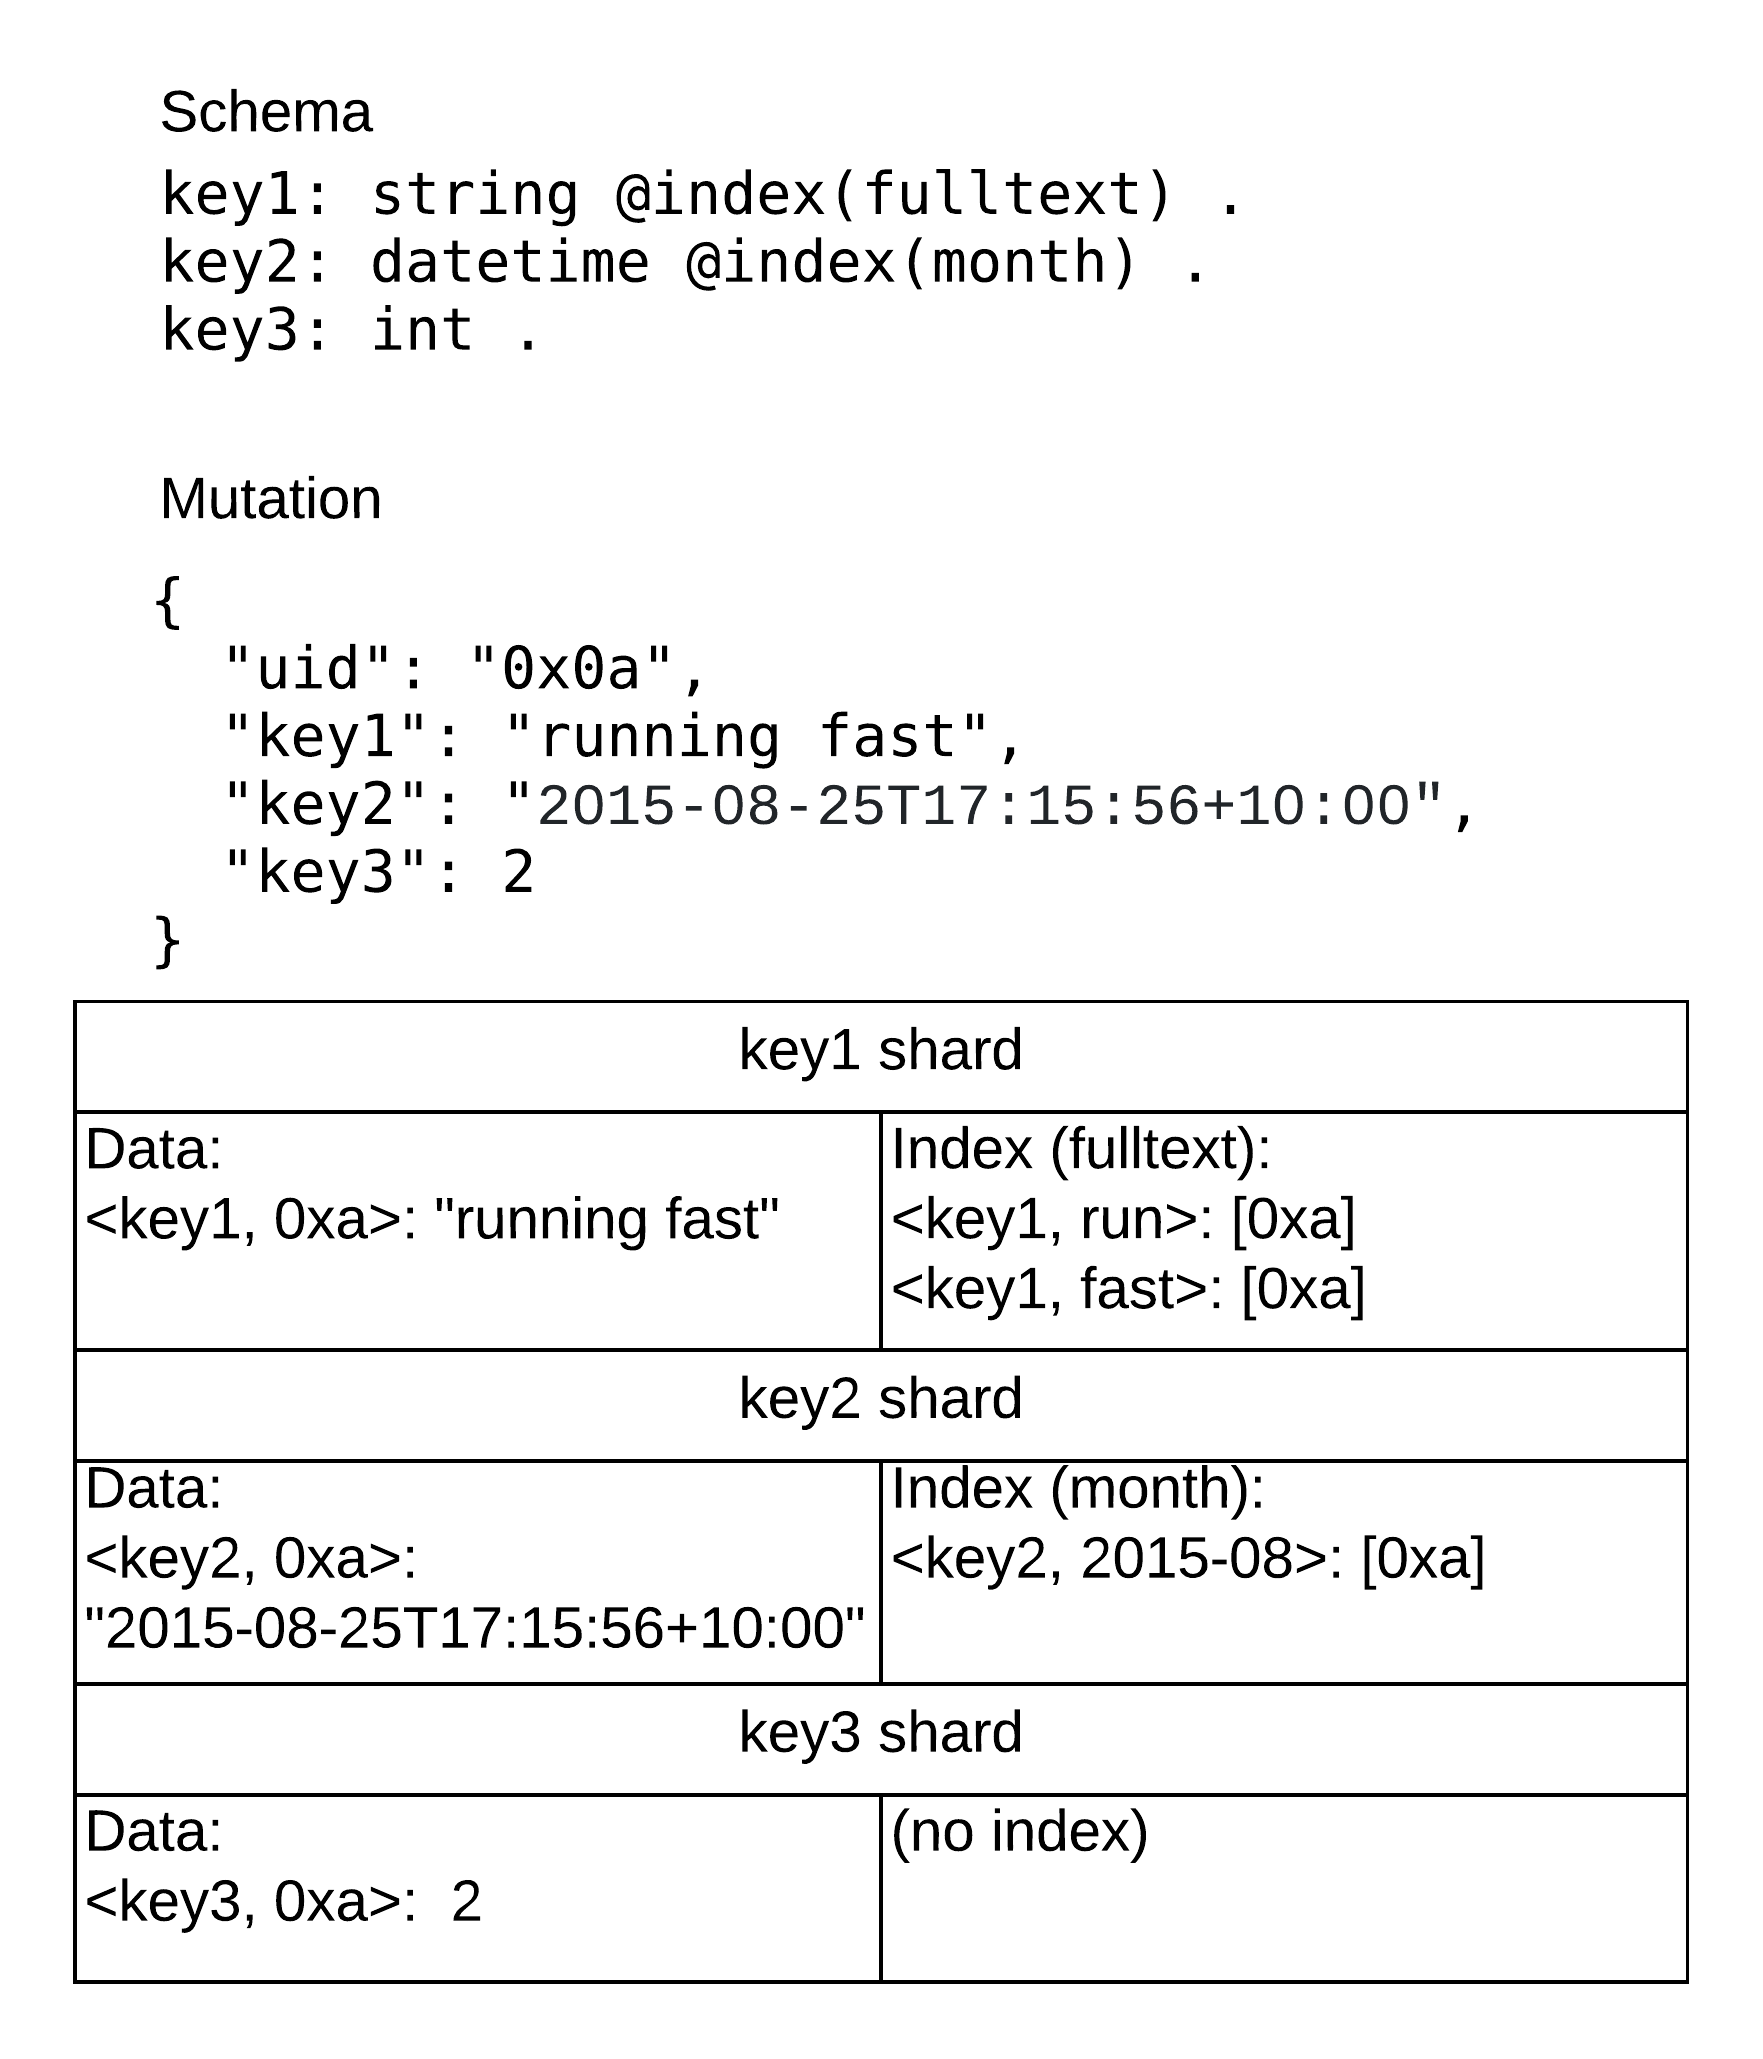
\includegraphics[scale=0.5]{datasharding.png}
\end{center}
\caption{Data sharding}
\end{figure}

\subsection{Data Rebalancing} \label{move}

As explained above, each shard contains a whole predicate in its entirety which
means Dgraph shards can be of uneven size. The shards not only contain the
original data, but also all of their indices. Dgraph groups contain many
shards, so the groups can also be of uneven size. The group and shard sizes are
periodically communicated to Zero. Zero uses this information to try to achieve
a balance among groups, using heuristics. Current one being used is just data
size, with the idea that equal sized groups would allow similar resource usage
across servers serving those groups. Other heuristics, particularly around query
traffic, could be added later.

To achieve balance, Zero would move shards from one group to another. It does so
by marking the shard read-only, then asking the source group to iterate over the
underlying key-values concurrently and streaming them over to the leader of the
destination group. The destination group leader proposes these key-values via
Raft, gaining all the correctness that comes with it. Once all the proposals
have been successfully applied by the destination group, Zero would mark the
shard as being served by the destination group. Zero would then tell source
group to delete the shard from its storage, thus finalizing the process.

While this process sounds pretty straighforward, there are many race and edge
conditions here which can cause transactional correctness to be violated as
shown by Jepsen tests \cite{jepsen}. We'll showcase some of these violations
here:

1. A violation can occur when a slightly behind Alpha server would think that it
is still serving the shard (despite the shard having moved to another group) and
allow mutations to be run on itself. To avoid this, all transactions states keep
the shard and the group info for the writes (along with their conflict keys as
we'll see in section \ref{txn}). The shard-group information is then checked by
Zero to ensure that what the transaction observes (via Alpha it talked to) and
what Zero has is the same -- a mismatch would cause a transaction abort.

2. Another violation happens when a transaction commits after the shard was put
into read-only mode -- this would cause that commit to be ignored during the
shard transfer. Zero catches this by assigning a timestamp to the move
operation. Any commits (on this shard) at a higher timestamp would be aborted,
until the shard move has completed and the shard is brought back to the
read-write mode.

3. Yet another violation can occur when the destination group receives a read
below the move timestamp, or a source group receives a read after it has deleted
the shard. In both cases, no data exists which can cause the reads to
incorrectly return back nil values. Dgraph avoids this by informing the
destination group of the move timestamp, which it can use to reject any reads
for that shard below it. Similarly, Zero includes a membership mark at which
the source Alpha must reach before the group can delete the shard, thus, every
Alpha member of the group would know that it is no longer servig the data before
deleting it.

Overall, the mechanism of membership information synchronization during a shard
move proved the hardest to get right with respect to transactional correctness.

\section{Indexing}

Dgraph is designed to be a primary database for applications. As such, it
supports most of the commonly needed indices. In particular, for strings, it
supports regular expressions, full-text search, term matching, exact and hash
matching index. For datetime, it supports year, month, day and hour level
indices. For geo, it supports nearby, within, etc. operations, and so on...

All these indices are stored by Dgraph using the same posting list format
described above. The difference between an index and data is the key. A data key
is typically \texttt{<predicate, uid>}, while an index key is
\texttt{<predicate, token>}. A token is derived from the value of the data,
using an index tokenizer.

Each index tokenizer supports this interface:

\begin{verbatim}
type Tokenizer interface {
  Name() string

  // Type returns the string representation of
  // the typeID that we care about.
  Type() string

  // Tokens return tokens for a given value. The
  // tokens shouldn't be encoded with the byte
  // identifier.
  Tokens(interface{}) ([]string, error)

  // Identifier returns the prefix byte for this
  // token type. This should be unique. The range
  // 0x80 to 0xff (inclusive) is reserved for
  // user-provided custom tokenizers.
  Identifier() byte

  // IsSortable returns true if the tokenizer can
  // be used for sorting/ordering.
  IsSortable() bool

  // IsLossy() returns true if we don't store the
  // values directly as index keys during
  // tokenization. If a predicate is tokenized
  // using a lossy tokenizer, we need to fetch
  // the actual value and compare.
  IsLossy() bool
}
\end{verbatim}

Every tokenizer has a globally unique identifier (\texttt{Identifier() byte}),
including custom tokenizers provided by operators. The tokens generated are
prefixed with a tokenizer identifier to be able to traverse through all tokens
belonging to only that tokenizer. This is useful when doing iteration for
inequality queries (greater than, less than, etc.). Note that inequality queries
can only be done if a tokenizer is sortable (\texttt{IsSortable() bool}). For
example, in strings, an exact index is sortable, but a hash index is not.

Depending upon which index a predicate has set in the schema, every mutation in
that predicate would invoke one or more of these tokenizers to generate the
tokens. Note that indices only operate on values, not objects. A set of
tokens would be generated with the before mutation value and another set
with the after mutation value. Mutations would be added to delete the
subject uid from the posting lists of before tokens and to add the subject
uid to the after tokens.

Note that all indices have object values, so they largely deal only in uids.
Indices in particular can suffer from high fan-out problem and are solved using
posting list splits described in the section \ref{storage}.

\section{Multiple Version Concurrency Control}

As described in section \ref{storage}, data is stored in posting list format,
which consists of postings sorted by integer ids.  All posting list writes are
stored as deltas to Badger on commit, using the commit timestamp. Note that
timestamps are monotonically increasing globally across the DB, so any future
commits are guaranteed to have a higher timestamp.

It is not possible to update this list in-place, for multiple reasons. One is
that Badger (and most LSM trees) writes are immutable, which plays very well
with filesystems and rsync.  Second is that adding an entry within a sorted list
requires moving following entries, which depending upon the position of the
entry can be expensive. Third, as the posting list grows, we want to avoid
rewriting a large value every time a mutation happens (for indices, it can
happen quite frequently).

Dgraph considers a posting list as a state. Every future write is then
stored as a delta with a higher timestamp. A delta would typically consist of
postings with an operation (set or delete). To generate a posting list, Badger
would iterate the versions in descending order, starting from the read
timestamp, picking all deltas until it finds the latest state.  To run a posting
list iteration, the right postings for a transaction would be picked, sorted by
integer ids, and then merge-sort operation is run between these delta postings
and the underlying posting list state.

Earlier iterations of this mechanism were aimed at keeping the delta layer
sorted by integer ids as well, overlaying it on top of the state to avoid doing
sorting during the reads --- any addition or deletion made would be consolidated
based on what was already in the delta layer and the state. These iterations
proved too complex to maintain for the team and suffered from hard to find bugs.
Ultimately, that concept was dropped in favor of a simple understandable
solution of picking the right postings for a read and sorting them before
iteration. Additionally, earlier APIs implemented both forward and backward
iteration adding complexity. Over time, it became clear that only forward
iteration was required, simplifying the design.

There are many benefits in avoiding having to regenerate the posting list state
on every write. At the same time, as deltas accumulate, the work of list
regeneration gets delegated to the readers, which can slow down the reads. To
find a balance and avoid gaining deltas indefinitely, we added a rollup mechanism.

\textbf{Rollups:} As keys get read, Dgraph would selectively regenerate the
posting lists which have a minimum number of deltas, or haven't been regenerated
for a while. The regeneration is done by starting from the latest state, then
iterating over the deltas in order and merging them with the state. The final
state is then written back at the latest delta timestamp, replacing the delta
and forming a new state.  All previous deltas and states for that key can then
be discarded to reclaim space.

This system allows Dgraph to provide MVCC. Each read is operating upon an
immutable version of the DB. Newer deltas are being generated at higher
timestamps and would be skipped during a read at a lower timestamp.

\begin{figure}[t]
\begin{center}
	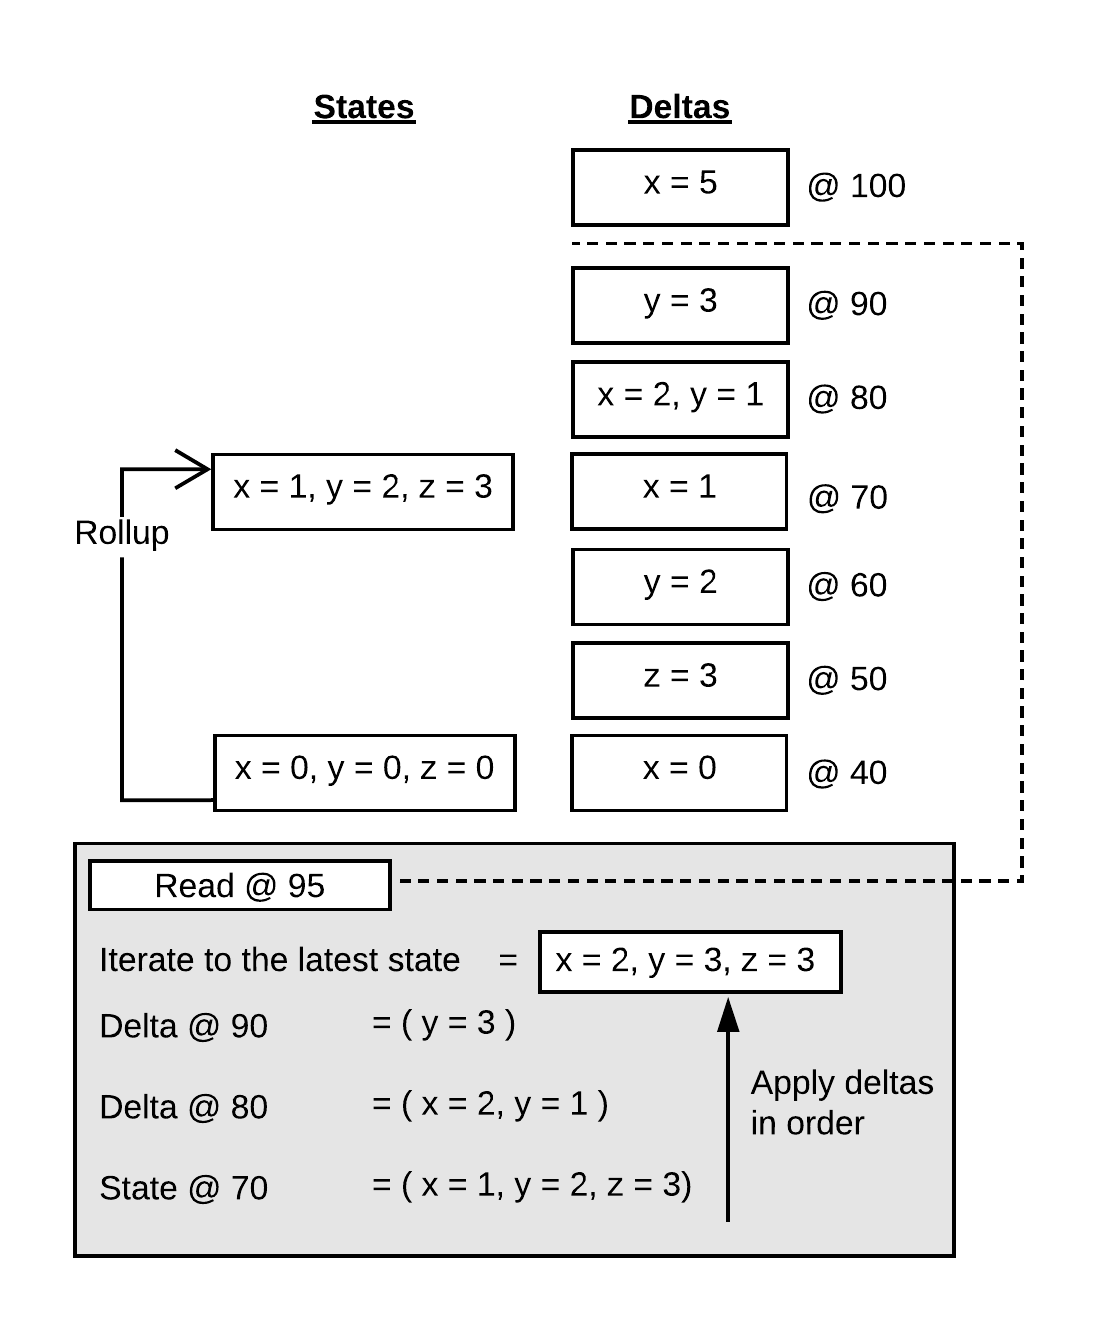
\includegraphics[scale=0.8]{mvcc.png}
\end{center}
\caption{MVCC}
\label{fig:mvcc}
\end{figure}

\section{Transactions} \label{txn}

Dgraph has a design goal of being simple to operate. As such, one of the goals
is to not depend upon any third party system. This proved quite hard to achieve
while providing high availability for not only data but also transactions.

While designing transactions in Dgraph, we looked at papers from Spanner
\cite{spanner}, HBase \cite{omid2}, Percolator \cite{peng} and others. Spanner
most famously uses atomic clocks to assign timestamps to transactions. This
comes at the cost of lower write throughput on commodity servers which don't
have GPS based clock sync mechanism. So, we rejected that idea in favor of
having a single Zero server, which can hand out logical timestamps at a much
faster pace.

To avoid Zero becoming a single point of failure, we run multiple Zero instances
forming a Raft group. But, this comes with a unique challenge of how to do
handover in case of leader relection.  Omid, Reloaded\cite{omid2} (referenced as
Omid2) paper handles this problem by utilizing \textit{external} system. In
Omid2, they run a standby timestamp server to take over in case the leader
fails. This standby server doesn't need to get the latest transaction state
information, because Omid2 uses Zookeeper\cite{zoo}, a centralized service for
maintaining transaction logs. Similarly, TiDB built TiKV, which uses a
Raft-based replication model for the key-values. This allows every write by TiDB
to automatically be considered highly-available.  Similarly,
Bigtable\cite{bigtable}, uses Google Filesystem\cite{gfs} for distributed
storage.  Thus, no direct information transfer needs to happen among the
multiple servers forming the quorum.

While this concept achieves simplicity in the database, we were not entirely
thrilled with this idea due to two reasons. One, we had an explicit goal of
non-reliance on any third-party system to make running Dgraph operationally
easier, and felt that a solution should be possible without pushing synchronous
replication within Badger (storage). Second, we wanted to avoid touching disk
unless necessary. By having Raft be part of the Dgraph process, we can find-tune
when things get written to state to achieve better efficiency. In fact, our
implementation of transactions don't write to DB state on disk until they are
committed (still written to Raft WAL).

We closely looked at HBase papers (\cite{omid1}, \cite{omid2}) for other ideas,
but they didn't directly fit our needs. For example, HBase pushed a lot of
transaction information back to the client, giving them critical information
about what they should or should not read to maintain the transactional
guarantees. This however, makes the client libraries harder to build and
maintain, something we did not like. On top of that, a graph query can touch
millions of keys in the intermediate steps, it's expensive to keep track of all
that information and propagate that to the client.

Aim for Dgraph client libraries was to keep as minimal state as possible to
allow open-source users unfamiliar with the internals of Dgraph to build
and maintain libraries in languages unfamiliar to us (for example, Elixir).

// TODO: Do I describe the first iteration?

We simply could not find a paper at the time which described how to build a
simple to understand, highly-available transactional system which could be run
without assuming that the storage layer is highly available. So, we had to come
up with a new solution. Our second iteration still faced many issues as proven by
Jepsen tests. So, we simplified our second iteration to a third one, which is as
follows.

\subsection{Lock-Free High Availability Transaction Processing}

Dgraph follows a lock-free transaction model. Each transaction pursues its
course concurrently, never blocking on other transactions, while reading the
committed data at or below its start timestamp. As mentioned before, Zero leader
maintains an Oracle which hands out logical transaction timestamps to Alphas.
Oracle also keeps track of a commit map, storing a conflict key $\rightarrow$ latest commit
timestamp. As shown in algorithm \ref{commit}, every transaction provides the
Oracle the list of conflict keys, along with the start timestamp of the
transaction. Conflict keys are derived from the modified keys, but are not the
same. For each write, a conflict key is calculated depending upon the schema.
When a transaction requests a commit, Zero would check if any of those keys has
a commit timestamp higher than the start timestamp of the transaction. If the
condition is met, the transaction is aborted. Otherwise, a new timestamp is
leased by the Oracle, set as the commit timestamp and conflict keys in the map
are updated.

\begin{algorithm}[t]
  \caption{Commit ($T_s, Keys$)}\label{commit}
	\begin{algorithmic}[1]
    \For{each key $k \in Keys$}
    \If {$lastCommit(k) > T_s$}
    \State $Propose(T_s \gets abort)$
    \State \Return
    \EndIf
		\EndFor
    \State $T_c \gets GetTimestamps(1)$
    \For{each key $k \in Keys$}
    \State $lastCommit(k) \gets T_c$
    \EndFor
    \State $Propose(T_s \gets T_c)$
	\end{algorithmic}
\end{algorithm}

% \begin{verbatim}
% Commit(startTs, conflictKeys):
%   for key in conflictKeys:
%     foundTs := Oracle.ConflictMap[key]
%     if foundTs > startTs:
%       return 0  // Found a conflict
%   // No conflicts found.
%   commitTs := leaseTimetamp(1)
%   for key in conflictKeys:
%     Oracle.ConflictMap[key] = commitTs
%   return commitTs
% \end{verbatim}

The Zero leader then proposes this status update (commit or abort) in the form
of a start $\rightarrow$ commit ts (where commit ts = 0 for abort) to the followers and
achieves quorum. Once quorum is achieved, Zero leader streams out this update to
the subscribers, which are Alpha leaders. To keep the design simple, Zero does
not push to any Alpha leader. It is the job of (whoever is) the latest Alpha
leader to establish an open stream from Zero to receive transaction status updates.

\begin{algorithm}[t]
  \caption{Watermark: Calculate DoneUntil ($T, isPending$)}\label{watermark}
	\begin{algorithmic}[1]
    \If {$T \notin MinHeap$}
    \State $MinHeap \gets T$
    \EndIf
    \State $ pending(T) \gets isPending $
    \State $curDoneTs \gets DoneUntil$
    \For{each $minTs \in MinHeap.Peek()$}
    \If {$pending(minTs)$}
    \State $break$
    \EndIf
    \State $MinHeap.Pop()$
    \State $curDoneTs \gets minTs$
		\EndFor
    \State $DoneUntil \gets curDoneTs$
	\end{algorithmic}
\end{algorithm}

Along with the transaction status update, Zero leader also sends out a
MaxAssigned timestamp. MaxAssigned is calculated using a Watermark algorithm
\ref{watermark}, which maintains a min-heap of all allocated timestamps, both
start and commit timestamps. As consensus is achieved, the timestamps are marked
as done and MaxAssigned gets advanced to the maximum timestamp up until which
everything has achieved consensus as needed. Note that start timestamps don't
typically need a consensus (unless lease needs to be updated) and get marked as
done immediately. Commit timestamps always need a consensus to ensure that Zero
group achieves quorum on the status of the transaction. This allows a Zero
follower to become a leader and have full knowledge of transaction statuses. This
ordering is crucial to achieve the transactional guarantees as we will see
below.

\begin{figure}[t]
\begin{center}
	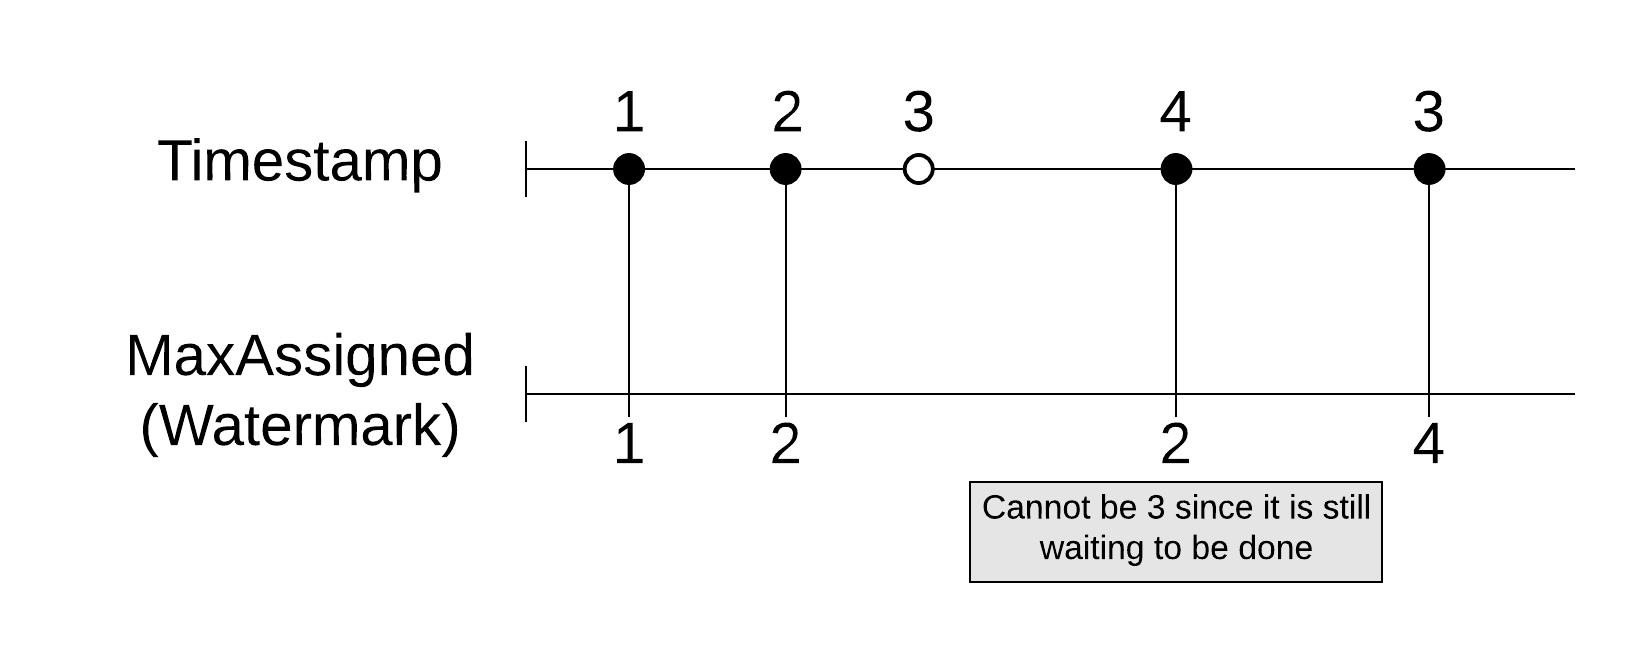
\includegraphics[scale=0.65]{maxassigned.png}
\end{center}
\caption{MaxAssigned watermark. Open circles represent and filled circles represent done. Start timestamps 1, 2, and 4 are immediately marked as done. Commit timestamp 3 begins and must have consensus before it is done. Watermark keeps track of the highest timestamp at and below which everything is done.}
\end{figure}

\begin{figure}[t]
\begin{center}
	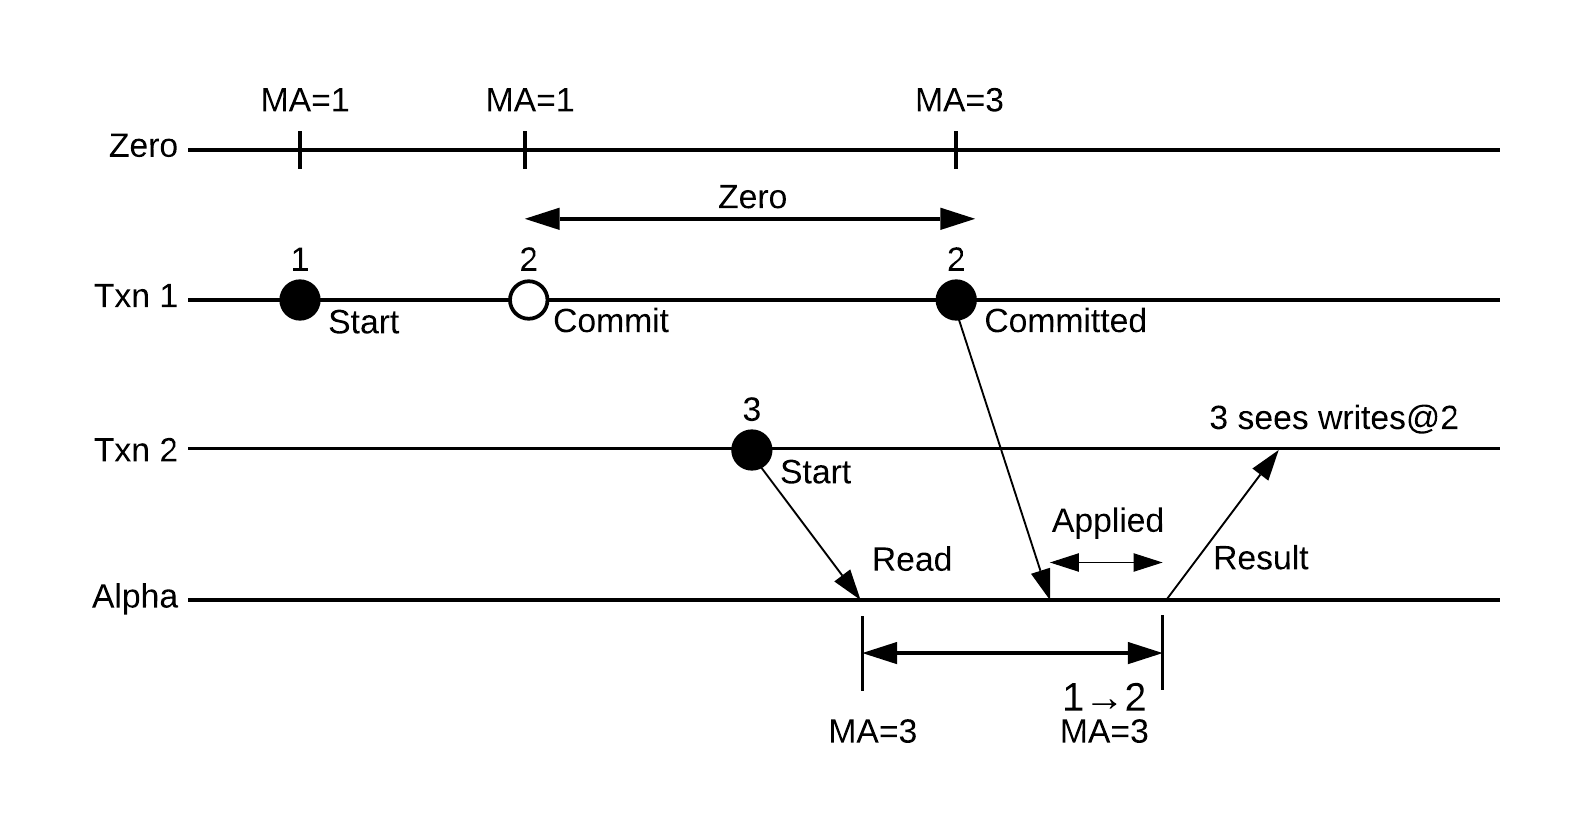
\includegraphics[scale=0.65]{maxassigned-derivation.png}
\end{center}
\caption{The MaxAssigned system ensures that linearizable reads. Reads at timestamps higher than the current MaxAssigned (MA) must block to ensure the writes up until the read timestamp are applied. Txn 2 receives start ts 3, and a read at ts 3 must acknowledge any writes up to ts 2.}
\end{figure}

Once Alpha leaders receive this update, they would propose it to their
followers, applying the updates in the same order. All Raft proposal
applications in Alphas are done serially. Alphas also have an Oracle, which
keeps track of the pending transactions. They maintain the start timestamp,
along with a transaction cache which keeps all the updated posting lists in
memory. On a transaction abort, the cache is simply dropped. On a transaction
commit, the posting lists are written to Badger using the commit timestamp.
Finally, the MaxAssigned timestamp is updated.

Every read or write operation must have a start timestamp. When a new query or
mutation hits an Alpha, it would ask Zero to assign a timestamp. This operation
is typically batched to only allow one pending assignment call to Zero leader
per Alpha. If the start timestamp of a newly received query is higher than the
MaxAssigned registered by that Alpha, it would block the query until its
MaxAssigned reaches or exceeds the start ts. This solution nicely tackles a
wide-array of edge case scenarios, including Alpha falling back or going behind
a network partition from its peers or just restarting after a crash, etc. In all
those cases, the queries would be blocked until the Alpha has seen all updates
up until the timestamp of the query, thus maintaining the guarantee of
transactions and linearizable reads.

For correctness, only Zero leader is allowed to assign timestamps, uids, etc.
There are edge cases where Zero followers would mistakenly think they're the
leaders and serve stale data --- Dgraph does multiple things to avoid these
scenarios.

1. If a Zero leadership changes, the new leader would lease out a range of
timestamps higher than the previous leader has seen.  However, an older commit
proposal stuck with the older leader can get forwarded to the new one. This can
allow a commit to happen at an older timestamp, causing failure of transactional
guarantees. We avoid this by disallowing Zero followers forwarding requests to
the leader and rejecting those proposals.

// TODO: We should have a membership section, which explains how membership
works and is transmitted to Alphas.

2. Every membership state update streamed from Zero requires a read-quorum
(check with Zero peers to find the latest Raft index update seen by the group).
If the Zero is behind a partition, for example, it wouldn't be able to achieve
this quorum and send out a membership update. Alphas expect an update
periodically and if they don't hear from the Zero leader after a few cycles,
they'd consider the Zero leader defunct, abolish connection and retry to
establish connection with a (potentially different) healthy leader.

\section{Consistency Model}

Dgraph supports MVCC, Read Snapshots and Distributed ACID transactions.  The
transactions are cluster-wide across universal dataset -- not limited by any key
level or server level restrictions. Transactions are also lockless.  They don’t
block/wait on seeing pending writes by uncommitted transactions. They can all
proceed concurrently and Zero would choose to commit or abort them depending on
conflicts.

Considering the expense of tracking all the data read by a single graph query
(could be millions of keys), Dgraph does not provide Serializable Snapshot
Isolation. Instead, Dgraph provides Snapshot Isolation, tracking writes which is
a much more contained set than reads.

Dgraph hands out monotonically increasing timestamps (represented by $T$) for
transactions (represented by $Tx$). Ergo, if any transaction $Tx_i$ commits
before $Tx_j$ starts, then $T_{commit}^{Tx_i} < T_{start}^{Tx_j}$. Any commit at
$T_{commit}$ is guaranteed to be seen by a read at timestamp $T_{read}$ by any
client, if $T_{read} > T_{commit}$. Thus, Dgraph reads are linearizable. Also,
all reads are snapshots across the entire cluster, seeing all previously
committed transactions in full.

As mentioned, Dgraph reads are linearizable. While this is great for correctness,
it can cause performance issues when a lot of reads and writes are going on
simultaneously. All reads are supposed to block until the Alpha has seen all the
writes up until the read timestamp. In many cases, operators would opt
for performance over achieving linearizablity. Dgraph provides two options for
speeding up reads:

1. A typical read-write transaction would allocate a new timestamp to the
client. This would update MaxAssigned which would then flow via Zero leader to
Alpha leaders and then get proposed. Until that happens, a read can't proceed.
Read-only transactions would still require a read timestamp from Zero, but Zero
would opportunistically hand out the same read timestamp to multiple callers,
allowing Alpha to amortize the cost of reaching MaxAssigned across multiple
queries.

2. Best-effort transactions are a variant of read-only transactions, which would
use an Alpha's observed MaxAssigned timestamp as the read timestamp. Thus, the
receiver Alpha does not have to block at all and can continue to process the
query. This is the equivalent of eventual consistency model typical in other
databases. Ultimately, every Dgraph read is a snapshot over the entire
distributed database and none of the reads would violate the snapshot guarantee.
\footnote{Note however that a typical Dgraph query could hit multiple Alphas in
various groups --- some of these Alphas might not have reached the read
timestamp (initial Alpha's MaxAssigned timestamp) yet. In those cases, the query
could still block until those Alphas catch up.}

\section{Replication}

Most updates to Dgraph are done via Raft. Let's start with Alphas which can push
a lot of data through the system. All mutations and transaction updates are
proposed via Raft and are made part of the Raft write-ahead logs. On a crash and
restart, the Raft logs are replayed from the last snapshot to bring the state
machine back up to the correct latest state. On the flip side, the longer the
logs, the longer it takes for Alpha to replay them on a restart, causing a start
delay. So, the logs must be trimmed by taking a snapshot which indicates that
the state up until that point has been persisted and does not need to be
replayed on a restart.

As mentioned above, Alphas write mutations to the Raft WAL, but keep them
in memory in a transaction cache. When a transaction is committed, the mutations
are written to the state at the commit timestamp. This means that on a restart,
all the pending transactions must be brought back to memory via the Raft WAL.
This requires a calculation to pick the right Raft index to trim the logs at,
which would keep all the pending transactions in their entirety in the logs.

One of the lessons we learnt while fixing Jepsen issues was that, to improve
debuggability of a complex distributed system, the system should run like clock
work. In other words, once an event in one system has happened, events in other
systems should almost be predictable. This guiding principle determined how we
take snapshots.

Raft paper allows leaders and followers to take snapshots independently of each
other. Dgraph used to do that but that brought unpredictability to the system
and made debugging much harder. So, keeping with the hard learnt lesson of
predictability principle, we changed it to make the leader calculate the
snapshot index and propose this result. This allowed leader and followers to all
take snapshot at the same index, exactly the same time (if they're generally
caught up). Further more, this group level snapshot event is then communicated
to Zero to allow it to trim the conflict map by removing all entries below the
snapshot timestamp. Following this chain of events in logs has improved
debuggability of the system dramatically.

Dgraph only keeps metadata in Raft snapshots, the actual data is stored
separately. Dgraph does not make a copy of that data during snapshot. When a
follower falls behind and needs a snapshot, it asks the leader for it and leader
would stream the snapshot from its state (Badger, just like Dgraph, supports
MVCC and when doing a read at a certain timestamp, is operating upon a logical
snapshot of the DB). In the previous versions, follower would wipe out its
current state before accepting the updates from the leader. In the newer
versions, leader can choose to send only the delta state update to the follower,
which can decrease the data transmitted considerably.

\section{High Availability and Scalability}

Dgraph's architecture revolves around Raft groups for update log serialization
and replication. In the CAP theorem, this follows CP, i.e. in a network
partition, Dgraph would choose consistency over availability. However, the
concepts of CAP theorem should not be confused with high availability, which is
determined by how many instances can be lost without the service getting
affected.

In a three-node group, Dgraph can loose one instance per group without causing
any measurable impact on the functionality of the database. However, loosing two
instances from the same group would cause Dgraph to block, considering all
updates go through Raft. In a five-node group, the number of instances that can
be lost without affecting functionality is two. We do not recommend running more
than five replicas per group.

Given the central managerial role of Dgraph Zero, one might assume that Zero
would be the single point of failure. However, that's not the case. In the
scenario where Zero follower dies, nothing changes really. If the Zero leader
dies, one of the Zero followers would become the leader, renew its timestamp and
uid assignment lease, pick up the transaction status logs (stored via Raft) and
start accepting requests from Alphas. The only thing that could be lost during
this transition are transactions which were trying to commit with the lost Zero.
They might error out, but could be retried. Same goes for Alphas. All Alpha
followers have the same information as the Alpha leader and any of the members
of the group can be lost without losing any state.

Dgraph can support as many groups as can be represented by 32-bit integer (even
that is an artificial limit). Each group can have one, three, five (potentially
more, but not recommended) replicas. The number of uids (graph nodes) that can
be present in the system are limited by 64-bit unsigned integer, same goes for
transaction timestamps. All of these are very generous limits and not a cause of
concern for scalability.

\section{Queries}

A typical Dgraph query can hit many Alphas, depending upon where the
predicates lie. Each query is sub-divided into tasks, each task
responsible for one predicate.

\subsection{Traversals}

Dgraph query tasks (henceforth referred to as tasks) are generally built around
the mechanism of converting uid list to matrix during traversal. The query can
have a list of uids to traverse, the execution engine would do lookups in Badger
concurrently to get the posting lists for each Uid (note that predicate is
always part of the task), converting each uid to a list. Thus, a task query
would return a list of Uid lists, aka UidMatrix. If the predicate holds a value
(example, predicate name), the UidList returns a list of values, aka
ValueMatrix. A predicate could allow only one uid/value, or allow multiple
uids/value. This mechanism works correctly in either of those scenarios. If the
posting list only has one uid/value, the resulting list would only have one
element. A matrix in this case would have a list of lists, each list with zero
or one element. Note that there's parity between the index of the Uid in list
and the index of the list in UidMatrix. So, Dgraph can accurately maintain the
relationships.

A ValueMatrix is typically the leaf in the task tree. Once we have values, we
just need to encode them in the results. However, a task with UidMatrix result would
typically have sub-tasks. Those sub-tasks would need a query UidList for
processing. Dgraph would merge-sort the UidMatrix into a single, sorted list of
Uids, which would be copied over to the sub-tasks. Each sub-task could similarly
run expand on the same or other predicates.

\subsection{Functions}

Dgraph also supports functions. These functions provide an easy way to query
Dgraph when the global uid space needs to be restricted to a small set (or even
a single uid). Functions also provide advanced functionality like regular
expressions, full-text search, equality and inequality over sortable data types,
geo-spatial searches, etc. These functions are also encoded into a task query,
except this time they don't start with a UidList. The task query instead
contains tokens, derived from the tokenizers corresponding to the index these
functions are using (as explained above). Most functions require some sort of
index to operate, for example, regular expression queries use trigram indexing,
geo-spatial queries uses S2-cell based geo indexing and so on...  As described
in section above, indexing keys encode predicate and token, instead of a
predicate and uid. So, the mechanism to fill up the matrix is the same as in any
other task query. Only this time, we use list of tokens instead of a list of
Uids as the query set.

\subsection{Filters}

The technique described above works for traversals. But, filters (intersections)
are a big part of user queries. Each task contains a UidList as a query and a
matrix as a result. Task also stores a resulting uid list, which can store a
uid set from the resulting UidMatrix. Depending upon whether filters are applied
or not, this uid set can be the same as merge-sorted UidMatrix or a subset of
it.

Filters are a tree in their own right. Dgraph supports AND, OR and NOT filters,
which can be further combined to create a complex filter tree. Filters typically
consist of functions which can ask for more information and are represented as
tasks.  These tasks execute in the same mechanism described above, but do one
additional thing. The tasks also contain the source list of Uids (the resulting
set from the parent task to which the filter is being applied to). This list of
uids is sent as part of the filter task. The task uses these uids to perform any
intersections at the destination server, returning only a subset of the results,
instead of retrieving all results for the task. This can significantly cut down
the result payload size while also allowing optimizations during filter task
execution to speed things up. Once the results are returned, the co-ordinator
server would stitch up the results using the AND, OR or NOT operators.

\subsection{Intersections}

The uid intersection itself uses three modes of integer intersection, choosing
between linear scan, block jump or binary search depending upon the ratio of the
size of the results and the size of the source UidList to provide the best
performance. When the two lists are of the same size, Dgraph
uses linear scan over both the lists. When one list is much
longer than other, Dgraph would iterate over the shorter list and do
binary lookups over the longer. For some range in between, Dgraph would iterate
over the shorter and do forward seeking block jumps over the longer list.
Dgraph's block based integer encoding mechanism makes all this quite efficient.

TODO: Talk about ACID.


\section{Future Work}

We had removed data caching from Dgraph due to heavy read-write contention, and
built a new, contention-free Go cache library to aid our reads. Work is underway
in integrating that with Dgraph. Dgraph does not have any query or response
caching --- such a cache would be difficult to maintain in an MVCC environment
where each read can have different results, based on its timestamp.

Sorted integer encoding and intersection is a hotly researched topic and there
is a lot of room for optimization here in terms of performance. As mentioned
earlier, work is underway in experimenting a switch to Roaring Bitmaps.

We also plan to work on a query optimizer, which can better determine the right
sequence in which to execute query. So far, the simple nature of GraphQL has
let the operators manually optimize their queries --- but surely Dgraph can do a
better job knowing the state of data.

Future work here is to allow writes during the shard move, which depending upon
the size of the shard can take some time.

TODO: Add a conclusion.

\section{Acknowledgments}

Dgraph wouldn't have been possible without the tireless contributions of its
core dev team and extended community. This work also wouldn't have been possible
without funding from our investors. A full list of contributors is present here:
\begin{center}
  {\tt github.com/dgraph-io/dgraph/graphs/contributors}
\end{center}

Dgraph is an open source software, available on
\begin{center}
  {\tt https://github.com/dgraph-io/dgraph}\\
\end{center}

More information about Dgraph is available on
\begin{center}
  {\tt https://dgraph.io}
\end{center}

{\footnotesize \bibliographystyle{acm}
  \bibliography{dgraph}}
\end{document}
